\documentclass[12pt]{report}
\usepackage[utf8]{inputenc}
\usepackage{graphicx}
\usepackage{subcaption}
\usepackage{setspace}
\usepackage{wrapfig}
\usepackage[font=small,labelfont=bf]{caption}

\doublespacing

\newcommand{\comment}[1]{}

\graphicspath{{Images/}}
\title{Thesis}
\author{John DeCorato}
\date{ }

\setlength{\parindent}{3em}
\setlength{\parskip}{1em}
 
\begin{document}
 
\maketitle
 
\tableofcontents

\pagebreak
\chapter{Introduction}

\begin{itemize}
	\item My project is 3-D sketching
	\item Important because when using current CAD software you need to know the dimensions of the final object. Not creative
	\item Different because we plan on focusing on recreating the environment and tools a designer uses
	\item Novel contributions are 3D layer system, reprojected pen styles 
\end{itemize}

\pagebreak
\chapter{Background / Related Work}

\section{Two-Dimensional Image Representation on Computers}

At it's most basic form, a sketch is an image drawn on a planar two-dimensional surface.
On computers, there are two methods or storing two dimensional images: raster graphics and vector graphics.
The underlying data structure has a large impact on the types of tools that can be designed to create and modify an image.

\subsection{Raster Graphics}

Raster graphics is an image format that uses a two-dimensional grid to represent each pixel in the image. 
A raster image is characterized by its width and height in pixels and by its color depth, the number of bytes per pixel, which determines the colors each pixel can represent.  
The reasoning behind representing images by this method is most computer monitors have bitmapped displays, where each pixel on the screen corresponds to a set of bits in memory telling the pixel what color to display. 
This allows for computers to easily display raster images, since the formats are largely the same.
\begin{figure}
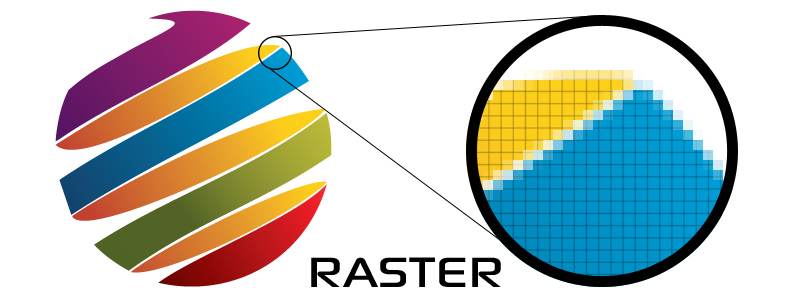
\includegraphics[width=\textwidth]{raster.jpg}
\caption{Zooming in on a Raster Graphics Image}
\end{figure}




Raster graphics are limited by the fact that the images it produces are resolution dependent. 
If you were to continuously zoom in on a raster image, eventually the image would suffer from image degradation. 
Pixel editing makes creating different tools for raster graphics easier, since the makers can just define how pixels are effected based on where the user is working. 
\begin{figure}
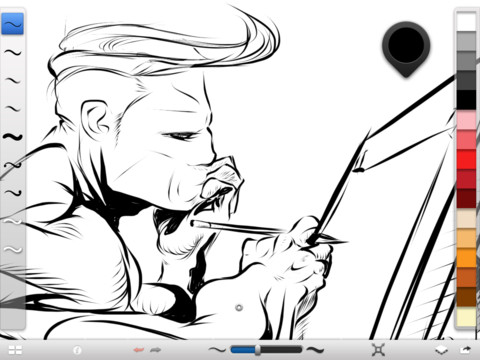
\includegraphics[width=\textwidth]{sketchbook.jpg}
\caption{Creating a Raster Image in Sketchbook}
\end{figure}



Examples of popular raster graphics software are Corel Painter, Adobe Photoshop, Microsoft's Paint.NET and MSPaint, the open-source GIMP software, and Autodesk's Sketchbook.

\comment{\subsubsection{Sketchbook Pro} http://www.autodesk.com/products/sketchbook-pro/features/all/gallery-view

Sketchbook Pro is a pixel drawing software application. It was originally made by Alias Systems Corporation, but is now owned and produced by Autodesk. Sketchbook is intended to simulate real-world art techniques such as pencil sketching, airbrushing, and painting.}

\subsection{Vector Graphics}

Vector graphics is the representation of an image by the use of geometrical primitives such as points, lines, curves, shapes and polygons.
Each of these primitives has a defined xy coordinate of the work space and determines the direction of the vector. 
Vectors can also be assigned a variety of properties such as its color, thickness, and fill.
Because of their mathematical nature, they are theoretically similar to three-dimensional computer graphics, but the term specifically refers to two-dimensional images; in part to distinguish them from raster graphics.
Vector graphics are primarily used for line art, images drawn with distinct straight or curved lines.
While there have been displays specialized in rendering them in the past, vector graphics in modern times are converted to raster graphics when used outside of vector specific editing tools.  

Vector graphics offer a number of advantages compared to raster images. 
First, since vector graphics are based on mathematical expressions, zooming in on the image does not cause image degradation like in raster graphics; the image will remain smooth. 
Second, objects made using vector graphics are independent from their visual representation.
This allows for the editing of primitives after they have been put inside of a vector graphics workspace.
For example, if I were to place a circle on top of a square in a raster graphics image, and then attempt to move the circle, there would be a circle-shaped hole in the square beneath.
This is because the raster image has no knowledge of the shapes, or shape depth, in the image, just the colors at each pixel.
However, in a vector image, the square would be unaffected..

\begin{figure}

\includegraphics[width=\textwidth]{vector.jpg}
\caption{Zooming in on a Vector Graphics Image}
\end{figure}

\subsection{Adaptive Distance Fields: Mischief} https://www.madewithmischief.com/

Mischief is a pseudo-vector graphics editor created by Made With Mischief, now owned by The Foundry. 
Although its systems are based on vector graphics, it does not allow for the precise editing of curves as seen in traditional vector graphics programs such as Adobe Illustrator. 
Instead it attempts to use vector graphics to simulate real world art techniques, like Sketchbook does.
This is possible by using a data-structure called Adaptive Distance Fields, which stores vectors in a tree data structure instead of the traditional vector format.
Since the tree data structure ends up looking like a pseudo-raster, raster brushes and pens can be implemented in this system by just telling it what shapes go inside of the data structure.
Adaptive Distance Fields also greatly reduce the storage size of large scale vectors, making it possible for the implementation of their infinite canvas; their infinitely zoom-able, translatable workspace. 
This allows for incredibly detailed and large scale.

\textbf{TODO:} Add examples of the infinite canvas (bug Nick)


\section{3-D Modeling in CAD}

Rhino

AutoCAD

Maya / 3DMAX

Sketchup

\section{3-D Sketching in CAD}

Talk abouw how people have tried to bring 3-D sketching to computers

\subsection{CATIA Natural Sketch}

Natural Sketch is a feature inside of the CATIA modeling software by Dassault Systemes. Natural Sketch allows the user to draw on a virtual plane, a 3-D model, and the plane where the screen lies in the 3D environment. It features the abilities to alter the pen style, alter the number of control points used to make the post sketch curve, automatically change the camera view to align with the drawing plane if one is being used, copy and alter individual strokes, and generate models from the 3-D sketch.

\begin{figure}

\begin{subfigure}{\textwidth}
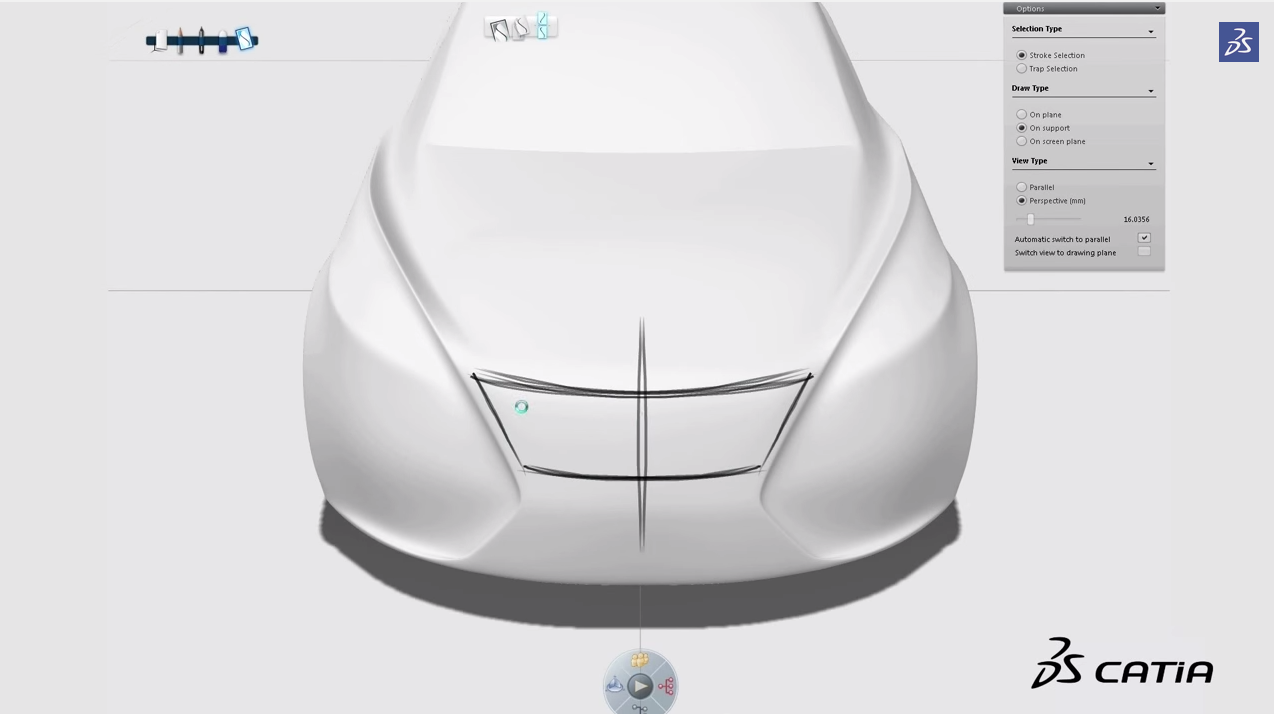
\includegraphics[width=\textwidth]{CATIA1}
\caption{Beginning the sketch}
\end{subfigure}
\begin{subfigure}{\textwidth}
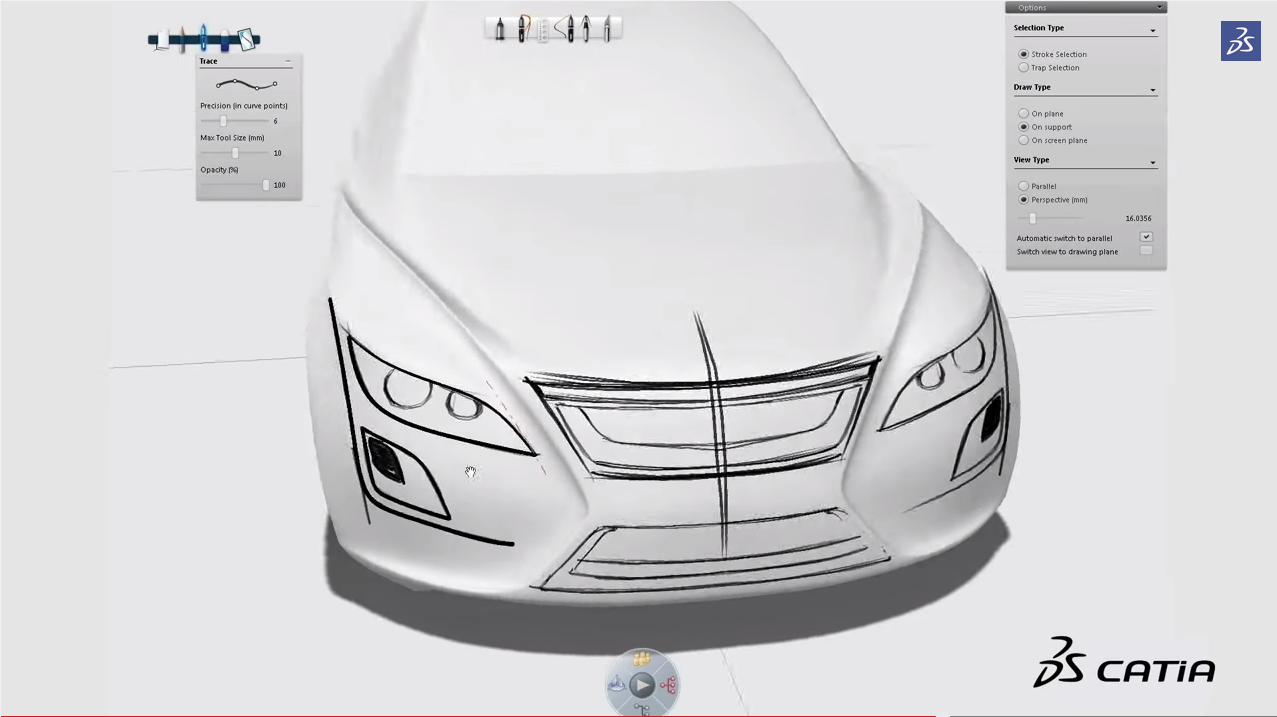
\includegraphics[width=\textwidth]{CATIA2}
\caption{Finishing the sketch}
\end{subfigure}

\caption{Using Natural Sketch to Add Detailing to a Car}
\end{figure}


\subsection{ILoveSketch / EverybodyLovesSketch}

EverybodyLovesSketch is a 3D curve sketching system from the University of Toronto's Dynamic Graphics Project Lab. It features a pen based gesture system, allowing the user to execute functions using rapid strokes, circles, and other defined gestures. Other features include dynamic sketch plane selection, single view definition of arbitrary extrusion vectors, multiple extruded surface sketching, copy-and-project of 3D curves, free-form surface sketching, and an interactive perspective grid. This project is based off of previous work by the same lab, ILoveSketch, which is the base 3D sketching functionality of the EverybodyLovesSketch project.

\subsection{Hyve 3D}

\begin{figure}

\begin{subfigure}{\textwidth}
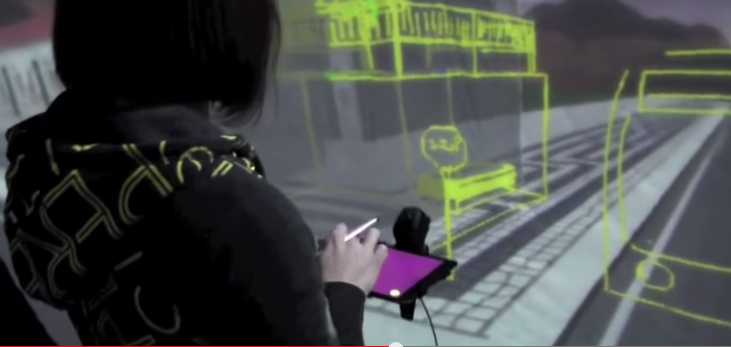
\includegraphics[width=0.9\linewidth]{Hyve3D1}
\caption{Using the tablet to draw}
\end{subfigure}
\begin{subfigure}{\textwidth}
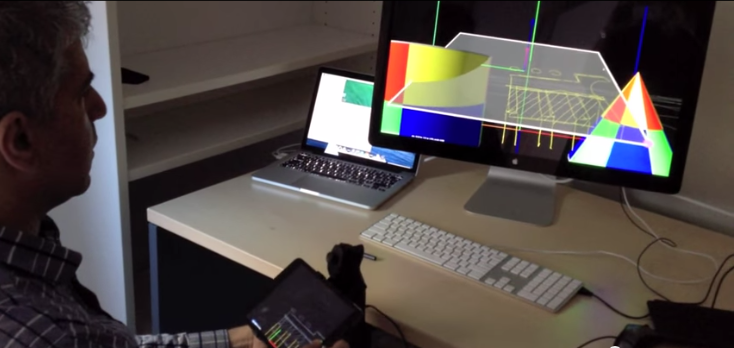
\includegraphics[width=0.9\linewidth]{Hyve3D2}
\caption{Manipulating the drawing plane}
\end{subfigure}

\caption{Examples of Hyve 3-D in use}
\end{figure}

Hyve 3D is an infinite virtual sketching environment from the University of Montreal. It uses two screens; a computer monitor to show the 3-D environment, and an iPad to draw. The sketching plane represented by the iPad is shown in the virtual environment, and is manipulated by moving and rotating the iPad in the real world. The user then pins the sketch plane in place and proceeds to draw at leisure. The advantage of this system is that it combines real world manipulation with virtual representation, eliminating the need for complex user interfaces and gestures. The disadvantage is that this kind of movement has no one-to-one feedback between the real world and the virtual, meaning that it is difficult to judge how your movements of the iPad effect the drawing place without confirming it visually.



\section{Other Work in 3-D Sketching}

Other forms of 3D content creation

Augmented Reality In-Situ 3D Sketching of Physical Objects $http://creativemachines.cornell.edu/papers/IUI09_Yee.pdf$

\subsection{Gravity} http://gravitysketch.com/

Gravity is an augmented reality 3D sketching tool using a tablet as the sketch base and a wearable screen to show the sketch. The tablet acts as a drawing plane, while the sketch can be moved via a set of controls on the tablet. The main idea is similar to Hyve 3D, in that you always draw in 2-D while you use your own sense of depth and position to understand what you are drawing, allowing for 3-D sketching without the use of perspective drawing. The difference is that this system allows you to use real world depth cues to augment your understanding of the virtual 3-D environment.

Sketch http://graphics.cs.brown.edu/research/sketch/

Polyes Q1 Pen http://technabob.com/blog/2014/12/29/polyes-q1-3d-sketching-pen/

\subsection{3-D Media Interaction}

Interacting with 3-D Media using modern input devices

Gestures vs. Postures: ‘Gestural’ Touch Interaction in 3D Environments 

\begin{verbatim}
$http://tobias.isenberg.cc/personal/papers/Isenberg_2012_GPG.pdf$
\end{verbatim}
A Survey of Interaction Techniques for Interactive 3D Environments http://www.grey-eminence.org/papers/EG2013-STAR.pdf

Interaction with 3-D environments using Multitouch Screens $http://www.researchgate.net/publication/236304194_Interaction_with_3D_Environments_using_Multi-Touch_Screens$

\pagebreak
\section{Input}

\begin{itemize}
\item Basic input chapter
\item Goal is to discuss where we are at in screen-based HCI
\item Hardware overview and methods, as well as gesture diagrams, use cases, etc
\end{itemize}
\subsection{Pen}

Discusses how people have attempted to solve HCI problems with pen input, as well as hardware and how the pen works 
Pen Based Interaction 
\begin{verbatim}
$http://www.academia.edu/2236260/Pen-based_Interaction_-_Next_Generation_User_Interfaces_WE-DINF-15756_$
\end{verbatim}
Pen-based User Interface 
\begin{verbatim}
$http://ieeexplore.ieee.org/stamp/stamp.jsp?tp=&arnumber=1349146$
\end{verbatim}
Experimental Analysis of Mode Switching Techniques in Pen-based User Interfaces http://research.microsoft.com/en-us/um/people/kenh/papers/p226-li.pdf
\subsection{Touch}

\subsection{Gesture}

\begin{figure}
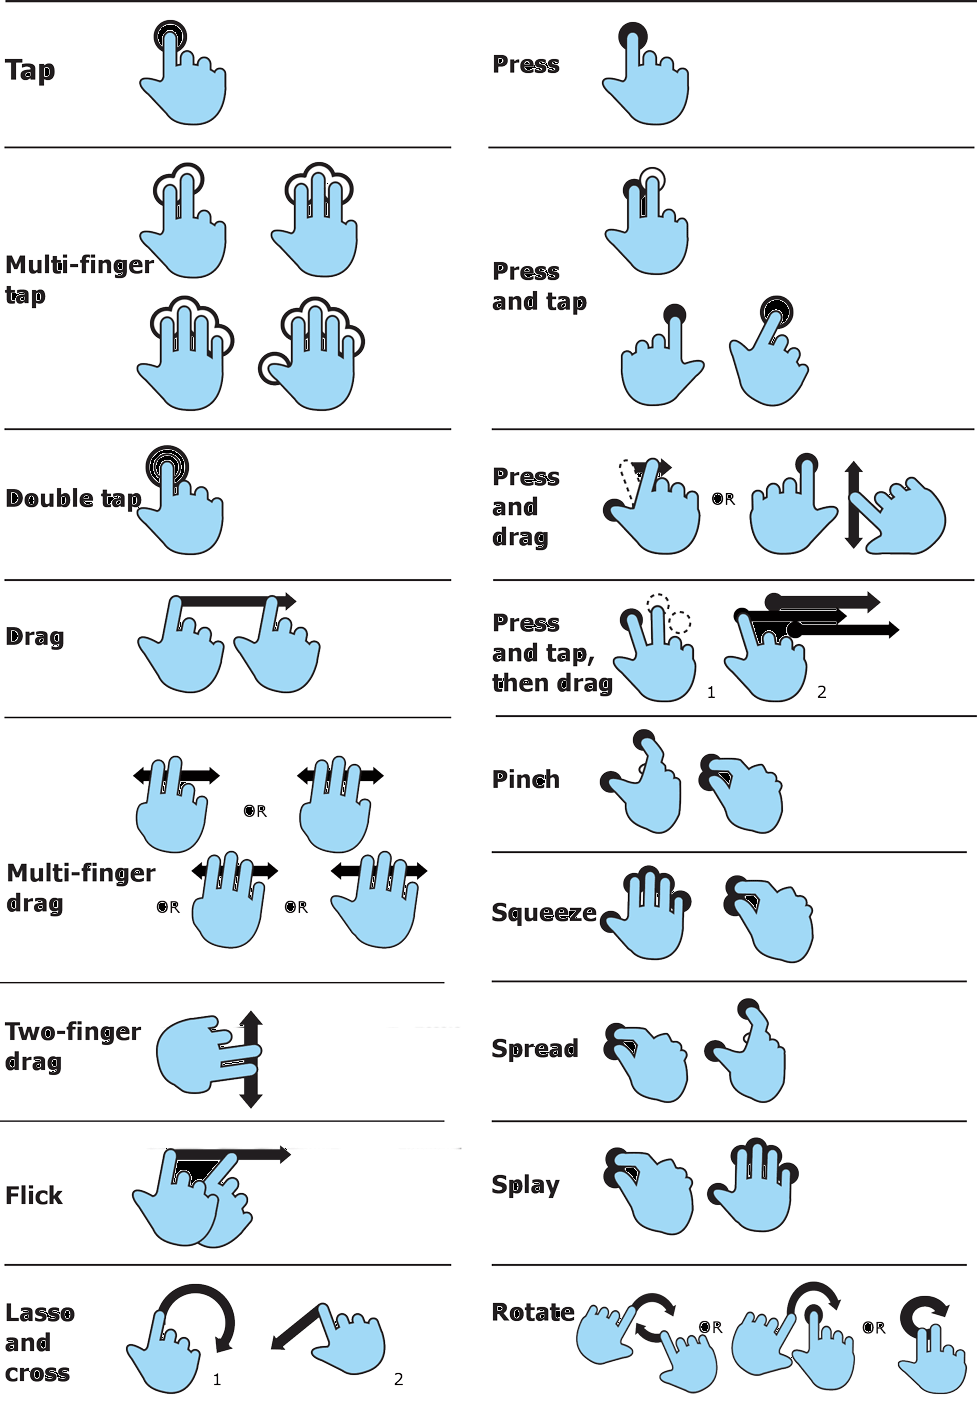
\includegraphics[width=0.9\linewidth]{GestureLibrary}
\caption{Touch Gesture Library}
\end{figure}
\begin{figure}
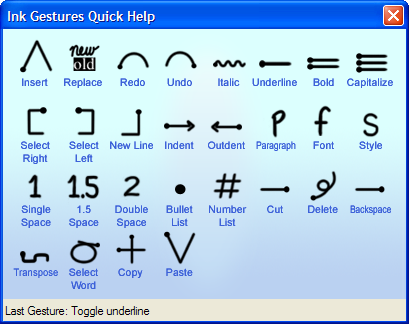
\includegraphics[width=0.9\linewidth]{pengestures}
\caption{Example Pen Gestures}
\end{figure}

\pagebreak

\chapter{Strokes, the Base of the Sketch}

\begin{itemize}
\item Spline talk chapter
\item Go over the inverse spline equation and the math behind the optimization
\item Get into 2-D to 3-D projection of strokes, and storage
\end{itemize}

\begin{figure}
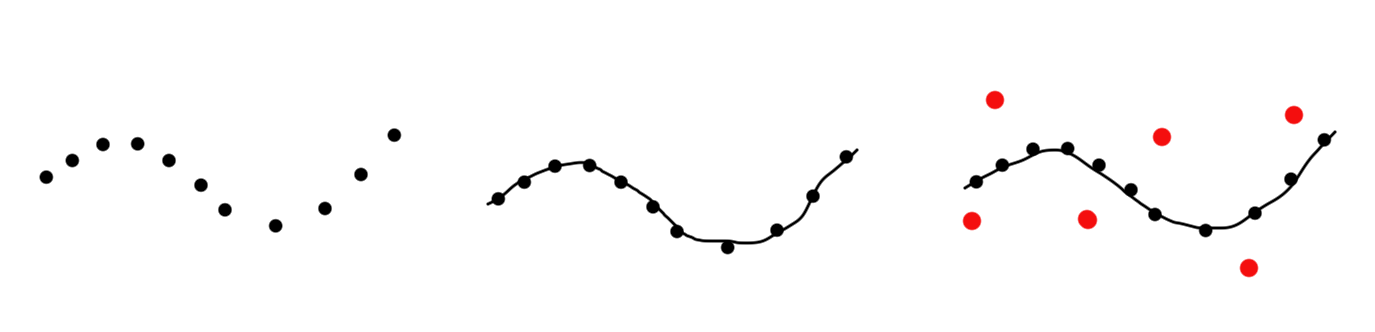
\includegraphics[width=0.9\linewidth]{CreatingACurve}
\caption{Rough Diagram of Optimizing a Curve using Control Points}
\end{figure}

Curve Global Interpolation http://www.cs.mtu.edu/~shene/COURSES/cs3621/NOTES/INT-APP/CURVE-INT-global.html

Smooth Spline Through Prescribed Points https://www.particleincell.com/2012/bezier-splines/

\section{Creating a Stroke}
\begin{itemize}
\item user inputs a series of points on the screen
\item storing all points too expensive, need to optimize
\item solution: create a curve based on the points that is defined by a smaller set of control points
\end{itemize}

\section{Definition of Splines}

Math goes here

\section{Inverse Spline Calculation}
Math goes here

\pagebreak
\chapter{Sketching in 3-D}

\begin{itemize}
\item Discuss how we get from the last chapter to 3-D sketching
\item Discuss Ray Casting and drawing surfaces
\item show system
\end{itemize}

\begin{figure}
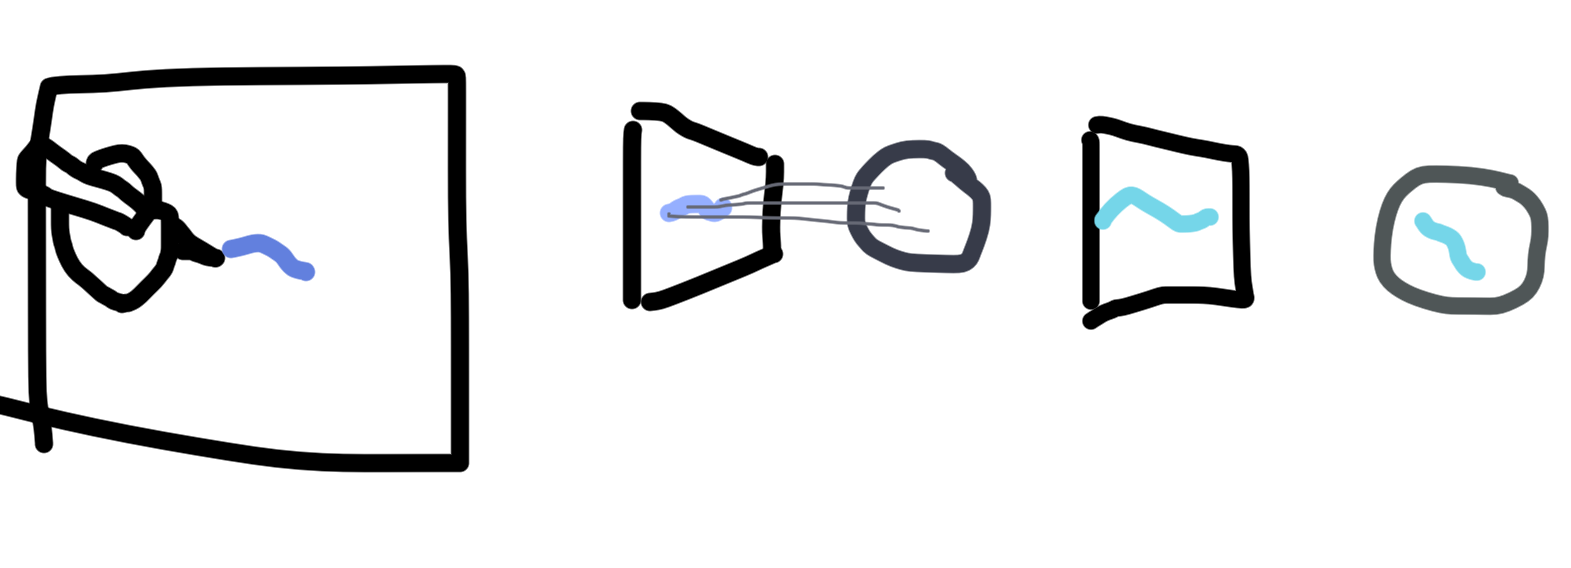
\includegraphics[width=0.9\linewidth]{StrokeProjection}
\caption{Rough Diagram of Projecting Stroke onto Drawing Surface}
\end{figure}

\section{Ray Casting}

\subsubsection{Acceleration Structure}
\begin{figure}[h]
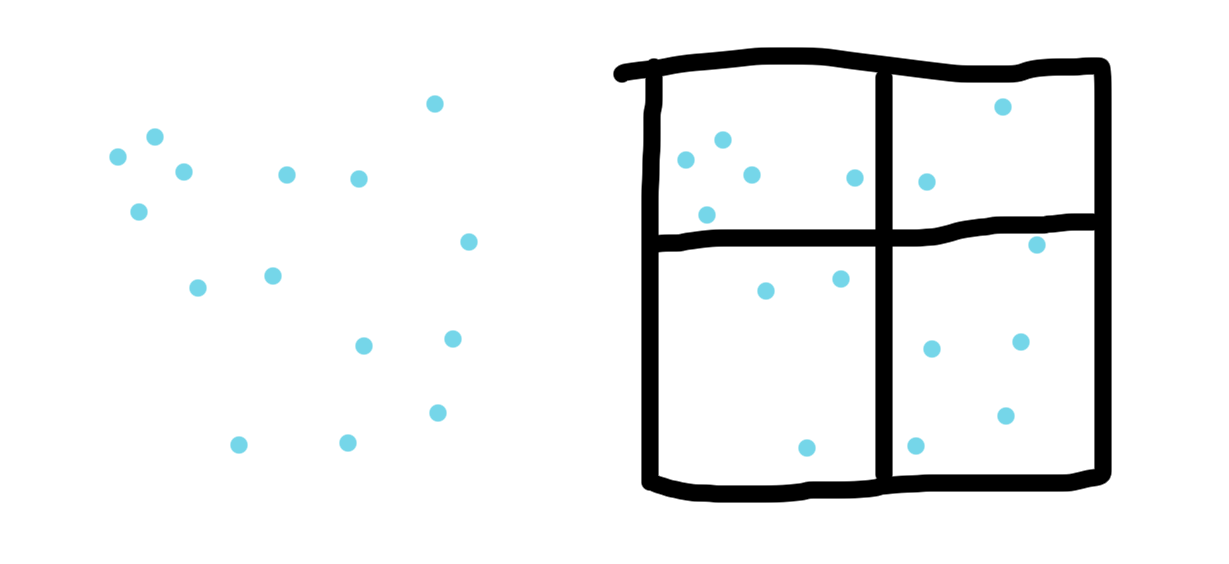
\includegraphics[width=0.9\linewidth]{AccelerationStructureExample}
\caption{Creating an Acceleration Structure}
\end{figure}
\subsubsection{Intersection}
Math goes here (Ray triangle intersection, Ray plane intersection, More in appendix? Reference?)
\subsection{Implementation}
\begin{itemize}
\item Display algorithm used
\item Discuss storage of strokes? (might not be particularly special)
\end{itemize}

\pagebreak
\chapter{Displaying Strokes}
Pen Styles section. This is getting complicated to the point that I think it needs it's own chapter
\begin{itemize}
\item Discuss reprojection of strokes into 2 space
\item Discuss pen styles and how pen styles are created (probably input reprojected 2D curve to geometry shader)
\item Discuss the what the actual styles are and the math behind them (possible appendix material after discussing one or two)
\end{itemize}
\pagebreak
\chapter{Usability and Feel: Bringing Physical Tools to the Virtual World}
\begin{itemize}
\item UX chapter
\item talk about how people actually use the system tools
\item talk about random quality of life features (page turning between layers, whatever else we come up with)
\end{itemize}
\section{Interacting with the 3D environment}
How do you move around the environment? How do you control things?
\section{Combining Pen and Touch}
Discus modality of system
\begin{figure}[h]
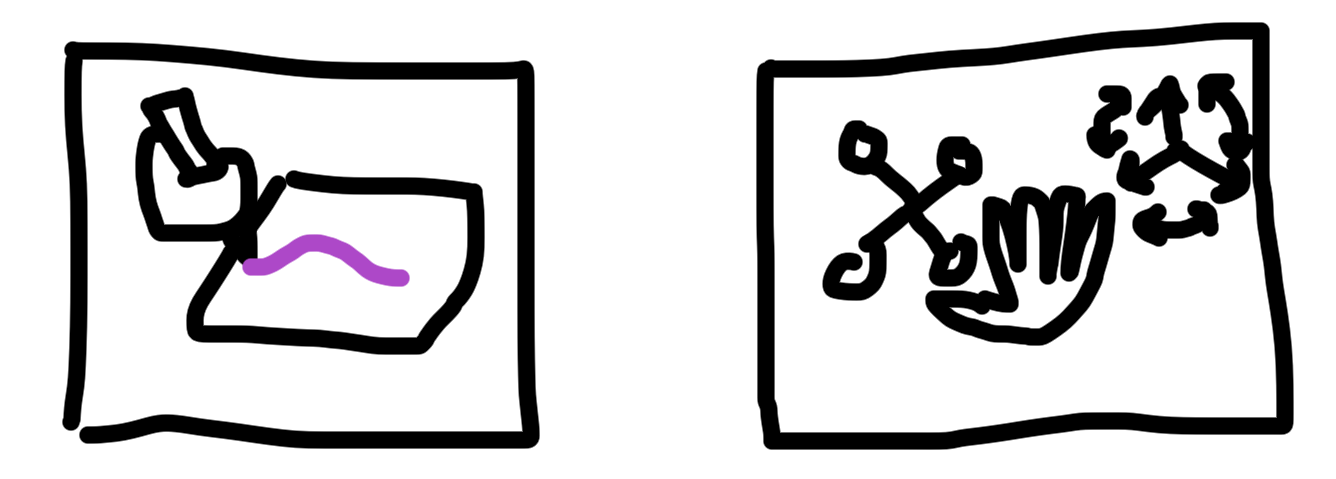
\includegraphics[width=0.9\linewidth]{Duality}
\caption{System Duality}
\end{figure}
\section{Turning the Page}
\begin{figure}[h]
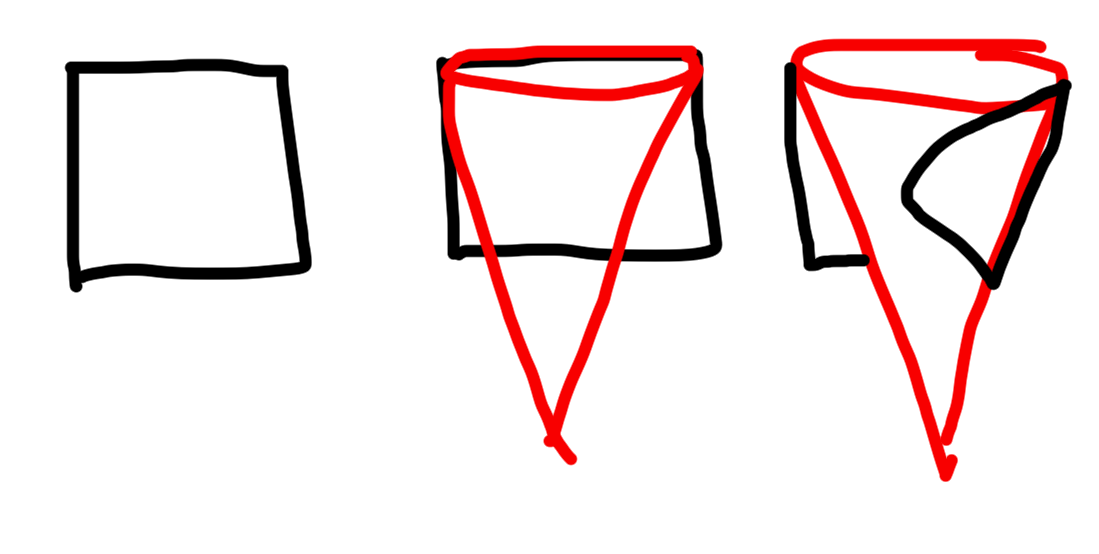
\includegraphics[width=0.9\linewidth]{TurningThePage}
\caption{Rough Diagram of math behind page turn}
\end{figure}
\begin{itemize}
\item Add reference to paper
\item show math
\end{itemize}


\pagebreak

\chapter{Conclusion}
Summary of everything goes here. More images of the system in use and example use cases.
\end{document}